\documentclass[conference]{IEEEtran}

\usepackage[utf8]{inputenc}
\usepackage[T1]{fontenc}
\usepackage[spanish]{babel}
\usepackage{amsmath,amssymb}
\usepackage{graphicx}
\usepackage{booktabs}
\usepackage{cite}
\usepackage{tikz}
\usetikzlibrary{positioning,calc,arrows.meta,babel}

\begin{document}
	
	\title{Optimizaci\'on metaheur\'istica de la configuraci\'on de extracci\'on de m\'etricas en fichas de modelos de Hugging Face}
	
	\author{\IEEEauthorblockN{Juan Felipe Gallo}
		\IEEEauthorblockA{Maestr\'ia en Ingenier\'ia, Universidad de Antioquia, Medell\'in, Colombia\\
			Metaheur\'istica 2026-01, Entrega 3}}
	
	\maketitle
	
	\begin{abstract}
		Se optimiza la configuraci\'on de la etapa de extracci\'on de m\'etricas de desempe\~no de un \emph{pipeline} ETL sobre fichas de modelos de Hugging Face: qu\'e reglas de un cat\'alogo activar, en qu\'e orden de prioridad y con qu\'e umbral de validaci\'on, para maximizar el $F_1$ macro por tarea con a lo sumo $K$ reglas, precisi\'on m\'inima de 0,90 y un tiempo m\'aximo por ficha. Se implementa GRASP con b\'usqueda local de cinco movimientos y memoria de evaluaciones, y se compara con un voraz constructivo, b\'usqueda aleatoria y enumeraci\'on exacta. En una instancia de 12 reglas con $K=4$, GRASP alcanza el \'optimo exacto (0,316) en las cinco r\'eplicas. En el cat\'alogo completo de 27 reglas empata con el voraz y supera a la b\'usqueda aleatoria con el mismo presupuesto. En validaci\'on cruzada agrupada por organizaci\'on, GRASP y el voraz no se distinguen (0,303 frente a 0,311, desviaci\'on cercana a 0,14). Una muestra manual de 36 fichas sin referencia da una precisi\'on del 100\,\% (IC 95\,\%: 90,4--100), casi toda en formato AutoTrain. Aplicada a los 1.664 modelos sin m\'etricas, la configuraci\'on optimizada de GRASP con $K=6$ recupera menos de 30, mientras que usar todas las reglas recupera 1.386 (83\,\%): la configuraci\'on ajustada sobre la referencia no se transfiere a esa poblaci\'on.
	\end{abstract}
	
	\begin{IEEEkeywords}
		metaheur\'isticas, GRASP, extracci\'on de informaci\'on, fichas de modelo, optimizaci\'on combinatoria.
	\end{IEEEkeywords}
	
	\section{Implementaci\'on}
	
	La implementaci\'on sigue el dise\~no de la Entrega 2 y se organiza en los m\'odulos de la Fig.~\ref{fig:comp}. El m\'odulo \texttt{evidence} contiene los analizadores de texto y \texttt{gold} la normalizaci\'on de nombres y la comparaci\'on con la referencia; \texttt{rules} define el cat\'alogo de 27 reglas. \texttt{evaluator} contiene \texttt{Instance}, que precalcula y guarda las salidas de las reglas y eval\'ua configuraciones. \texttt{baselines} aloja la clase \texttt{Objective} (aptitud, restricciones y cach\'e de evaluaciones) y los m\'etodos de comparaci\'on, y \texttt{grasp} implementa el algoritmo principal.
	
	\begin{figure}[t]
		\centering
		\begin{tikzpicture}[box/.style={draw,rounded corners=1pt,font=\scriptsize,align=center,minimum width=2.5cm,minimum height=0.62cm},node distance=5mm]
			\node[box] (evid) {analizadores\\(\texttt{evidence})};
			\node[box,right=8mm of evid] (data) {fichas y referencia\\(\texttt{gold})};
			\node[box,below=of evid] (rules) {27 reglas\\(\texttt{rules})};
			\node[box,below=of data] (inst) {\texttt{Instance}\\salidas guardadas};
			\node[box] (obj) at ($(rules)!0.5!(inst)+(0,-1.25)$) {\texttt{Objective}: aptitud,\\restricciones, cach\'e};
			\node[box,below=of obj,xshift=-1.45cm] (base) {\texttt{baselines}\\voraz, aleatoria, exacta};
			\node[box,below=of obj,xshift=1.45cm] (gr) {\texttt{grasp}\\construcci\'on + local};
			\draw[-{Stealth[length=1.8mm]}] (evid)--(rules);
			\draw[-{Stealth[length=1.8mm]}] (rules)--(inst);
			\draw[-{Stealth[length=1.8mm]}] (data)--(inst);
			\draw[-{Stealth[length=1.8mm]}] (inst)--(obj);
			\draw[-{Stealth[length=1.8mm]}] (obj)--(base);
			\draw[-{Stealth[length=1.8mm]}] (obj)--(gr);
		\end{tikzpicture}
		\caption{Componentes de la implementaci\'on y su relaci\'on.}
		\label{fig:comp}
	\end{figure}
	
	\subsection{Problema y representaci\'on}
	Cada ficha de modelo (\emph{model card}) \cite{mitchell} contiene m\'etricas en el bloque \texttt{model-index} y, con frecuencia, en tablas y l\'ineas del cuerpo. El ETL actual solo lee los metadatos y deja con m\'etricas 401 de 2.057 modelos (19,5\,\%). Se busca configurar una etapa de recuperaci\'on sobre el cuerpo de la ficha. Una soluci\'on es $x=(\pi,\theta)$: $\pi$ es una tupla ordenada de a lo sumo $K$ reglas distintas de un cat\'alogo de $m=27$ y $\theta\in\{1,100,1000\}$ es una cota superior de plausibilidad para los valores aceptados. Con $K=5$ el espacio tiene $3\sum_{k=1}^{5} m!/(m-k)!\approx 3{,}04\times10^{7}$ configuraciones.
	
	\subsection{Cat\'alogo de reglas}
	Una regla combina un analizador (l\'inea \texttt{nombre: valor}, fila de tabla \emph{markdown} o columna de tabla, tomando la \'ultima fila) con una subfamilia de m\'etricas: \texttt{clf\_basic}, \texttt{clf\_avg} (macro, micro y ponderadas), \texttt{rank} (nDCG, MAP, MRR), \texttt{at\_k}, \texttt{sim}, \texttt{rouge}, \texttt{bleu}, \texttt{reg} y \texttt{lm}. Son $3\times9=27$ reglas. Medido en esta implementaci\'on, procesar una ficha con todas cuesta 187\,ms, y la regla de fila de \texttt{at\_k} cuesta 67,8\,ms, m\'as del doble que cualquier otra.
	
	\subsection{Evaluaci\'on con memoria}
	La salida de cada regla sobre cada ficha se calcula una sola vez (73\,s para 27 reglas y 390 fichas), junto con las m\'etricas de referencia que acierta. Evaluar una configuraci\'on se reduce a combinar salidas guardadas y cuesta 3,3\,ms. La prioridad opera por m\'etrica: para cada ficha y nombre normalizado de m\'etrica, la primera regla de $\pi$ que la produce es su due\~na y aporta todos sus valores; las dem\'as se descartan para esa m\'etrica. Esto causa enmascaramiento: activar m\'as reglas puede empeorar el resultado. Una capa adicional de memoria guarda cada configuraci\'on evaluada y el presupuesto cuenta solo evaluaciones reales.
	
	Un valor extra\'ido acierta si el nombre can\'onico coincide con el de la referencia (por ejemplo, \texttt{ROUGE-1}$=$\texttt{rouge1}, \texttt{acc}$=$\texttt{accuracy}, \texttt{ndcg at 10}$=$\texttt{ndcg@10}) y el valor coincide con tolerancia relativa del 1\,\% (tambi\'en $\times100$ y $\div100$).
	
	\subsection{Funci\'on objetivo}
	Sea $T$ el conjunto de etiquetas de tarea (\texttt{pipeline\_tag}) y $F_{1,\tau}(x)$ el $F_1$ de la etiqueta $\tau$, con precisi\'on y cobertura agregadas en sus fichas. El objetivo es el $F_1$ macro, que pesa igual a cada tarea:
	\begin{equation}
		\bar F_1(x)=\tfrac{1}{|T|}\textstyle\sum_{\tau\in T}F_{1,\tau}(x).
	\end{equation}
	Se eligi\'o el macro porque dos tareas aportan 226 de las 390 fichas de referencia y el $F_1$ agregado deja poco que optimizar (0,885 con todas las reglas sin enmascarar). Su costo es que una etiqueta con una sola ficha pesa igual que una con cientos, lo que aumenta el ruido. Las restricciones son duras: precisi\'on global $P(x)\ge0{,}90$ y tiempo por ficha $t(x)\le t_{\max}$. Con la violaci\'on $v(x)=\max(0,\,0{,}90-P)+\max(0,\,t/t_{\max}-1)$, la aptitud es
	\begin{equation}
		f(x)=\begin{cases}\bar F_1(x) & v(x)=0,\\ -1-v(x) & v(x)>0,\end{cases}
	\end{equation}
	de modo que toda soluci\'on infactible vale menos que cualquier factible y $v$ orienta la b\'usqueda hacia la regi\'on factible. Una primera versi\'on penalizaba el tiempo con un factor peque\~no: los m\'etodos violaban la restricci\'on y esos resultados se descartaron.
	
	\subsection{GRASP}
	GRASP \cite{feo} repite construcci\'on y b\'usqueda local hasta agotar el presupuesto de evaluaciones. La \emph{construcci\'on} eval\'ua en cada paso todas las inserciones (regla, posici\'on) y elige al azar entre las que cumplen $f\ge f_{\max}-\alpha(f_{\max}-f_{\min})$; se detiene al llegar a $K$ reglas o si ninguna inserci\'on mejora. La \emph{b\'usqueda local} aplica mejor mejora sobre cinco movimientos: insertar, eliminar, reemplazar una regla, intercambiar dos posiciones y cambiar $\theta$. Devuelve la mejor configuraci\'on.
	
	\subsection{L\'ineas base}
	\emph{Voraz individual}: las $K$ reglas con mejor aptitud individual, en ese orden (l\'inea base propuesta en la Entrega 1). \emph{Voraz constructivo}: determinista, inserta en cada paso la regla y posici\'on que m\'as mejoran. \emph{B\'usqueda aleatoria}: configuraciones aleatorias con el mismo presupuesto. \emph{Enumeraci\'on exacta}: todas las ordenaciones de hasta $K$ reglas de un subcat\'alogo, para cada $\theta$.
	
	\section{Experimentos}
	
	\subsection{Instancias}
	Se descargaron 1.931 de 2.057 fichas; 126 no fueron accesibles (94 con error 403 y 32 con 404). La referencia es el \texttt{model-index} de 390 fichas con valores num\'ericos, oculto al extractor (se elimina el bloque YAML inicial). La partici\'on se hizo por organizaci\'on. El supuesto de representatividad de la Entrega 1 result\'o falso: las fichas con m\'etricas en el ETL son sobre todo de similitud de oraciones y extracci\'on de caracter\'isticas, y las 1.533 sin ellas son en su mayor\'ia AutoTrain. Por eso se a\~nadi\'o una muestra manual de 36 fichas sin referencia, proporcional por etiqueta. Las instancias son:
	\begin{itemize}
		\item \textbf{Peque\~na con \'optimo exacto:} subcat\'alogo de 12 reglas, $K=4$.
		\item \textbf{Cat\'alogo completo:} 27 reglas, $K\in\{3,4,5,6\}$, con $t_{\max}\in\{30,50,80\}$\,ms o sin l\'imite.
		\item \textbf{Validaci\'on cruzada por organizaci\'on:} 5 pliegues balanceados por n\'umero de fichas (236, 39, 39, 38 y 38). Una sola organizaci\'on aporta 236 de las 390 fichas y forma el primer pliegue completo.
	\end{itemize}
	
	\subsection{Ajuste de par\'ametros}
	Se ajustaron $\alpha\in\{0;0{,}1;0{,}3;0{,}5;0{,}8\}$ y el presupuesto $\in\{500;1500;3000\}$ evaluaciones, con 6 semillas por combinaci\'on, sobre 338 fichas de entrenamiento ($K=5$, $t_{\max}=80$\,ms). El criterio fue la aptitud media (Tabla~\ref{tab:ajuste}). Se eligi\'o $\alpha=0{,}3$ y 3.000 evaluaciones (0,420). Con 500 evaluaciones no se completa una iteraci\'on (la primera cuesta unas 700). De 1.500 en adelante hay meseta, y para $\alpha\ge0{,}1$ la diferencia es menor que 0,004; $\alpha=0$ (voraz m\'as b\'usqueda local) queda ligeramente por debajo.
	
	\begin{table}[t]
		\centering
		\caption{Aptitud media de GRASP ($K=5$, 6 semillas, entrenamiento)}
		\label{tab:ajuste}
		\footnotesize
		\begin{tabular}{lccc}
			\toprule
			$\alpha$ & 500 & 1500 & 3000 \\
			\midrule
			0,0 & 0,386 & 0,398 & 0,398 \\
			0,1 & 0,355 & 0,418 & 0,418 \\
			0,3 & 0,347 & 0,416 & \textbf{0,420} \\
			0,5 & 0,347 & 0,416 & 0,420 \\
			0,8 & 0,343 & 0,418 & 0,418 \\
			\bottomrule
		\end{tabular}
	\end{table}
	
	\subsection{Protocolo}
	Presupuesto de 3.000 evaluaciones (1.000 en la instancia peque\~na). R\'eplicas: 5 semillas en la instancia peque\~na y con restricci\'on de tiempo, 10 en la curva de convergencia y 3 por pliegue en validaci\'on cruzada. Se reportan $\bar F_1$, precisi\'on, cobertura, tiempo y factibilidad. El hardware y los tiempos son los de esta implementaci\'on en Python.
	
	\subsection{Desviaciones respecto a la Entrega 1}
	El cat\'alogo tiene 27 reglas y no entre 40 y 60. Se probaron $K\in\{3,4,5,6\}$ y no $\{5,10,15\}$, y solo la precisi\'on m\'inima de 0,90 (no 0,85 y 0,95). La referencia son 390 fichas con valores num\'ericos y no 401, y la tabla de homologaci\'on se sustituy\'o por una normalizaci\'on can\'onica de nombres. No se escalaron subconjuntos de 50, 100 y 200 fichas ni subcat\'alogos de 20 y 40 reglas; en su lugar hay una instancia peque\~na con \'optimo exacto y una validaci\'on cruzada por organizaci\'on. La l\'inea base ya no es la cascada actual, que solo lee metadatos, sino los m\'etodos voraces y la b\'usqueda aleatoria sobre las mismas reglas. El supuesto de representatividad no se sostuvo, como se indic\'o arriba.
	
	\section{Resultados}
	
	\subsection{\'Optimo exacto}
	Con 27 reglas y $K=3$, la enumeraci\'on completa (54.837 configuraciones, 43\,s) da 0,264, que el voraz constructivo ya alcanza. En el subcat\'alogo de 12 reglas con $K=4$, el \'optimo exacto (75\,s) es 0,316; el voraz y GRASP lo alcanzan en las 5 r\'eplicas, y la b\'usqueda aleatoria con 1.000 evaluaciones logra 0,294 en promedio (0,274--0,306). Con $t_{\max}=50$\,ms, el \'optimo en esa instancia es 0,264.
	
	\subsection{Cat\'alogo completo}
	La Tabla~\ref{tab:k} compara m\'etodos sin l\'imite de tiempo. El voraz individual se estanca porque elige reglas que se solapan (0,199 con $K=3$ y $K=4$). El voraz constructivo y GRASP coinciden, y la b\'usqueda aleatoria queda por debajo. La cota superior (todas las reglas sin enmascarar) es 0,383.
	
	\begin{table}[t]
		\centering
		\caption{$\bar F_1$ por m\'etodo y $K$ (cat\'alogo completo)}
		\label{tab:k}
		\footnotesize
		\begin{tabular}{lcccc}
			\toprule
			$K$ & Voraz ind. & Voraz constr. & Aleatoria & GRASP \\
			\midrule
			3 & 0,199 & 0,264 & -- & -- \\
			4 & 0,199 & 0,316 & -- & -- \\
			5 & 0,242 & 0,340 & 0,286 & 0,340 \\
			6 & -- & 0,357 & 0,320 & 0,357 \\
			\bottomrule
		\end{tabular}
	\end{table}
	
	\subsection{Restricci\'on de tiempo}
	Sin l\'imite de tiempo, el voraz usa la regla de 67,8\,ms y llega a 0,340 con 81\,ms por ficha. La Tabla~\ref{tab:t} muestra el compromiso con $K=5$; todas las soluciones son factibles. GRASP iguala al voraz con 30 y 50\,ms, y con 80\,ms es ligeramente mejor (0,289 frente a 0,285) usando 54\,ms en lugar de 78\,ms. A 80\,ms el voraz tambi\'en cae por debajo de lo que logra a 50\,ms (0,285 frente a 0,288): no cabe la regla cara y cae en una combinaci\'on peor.
	
	\begin{table}[t]
		\centering
		\caption{$\bar F_1$ y tiempo medio por ficha con $K=5$ (5 semillas)}
		\label{tab:t}
		\footnotesize
		\begin{tabular}{lcccccc}
			\toprule
			& \multicolumn{2}{c}{Voraz constr.} & \multicolumn{2}{c}{Aleatoria} & \multicolumn{2}{c}{GRASP} \\
			$t_{\max}$ & $\bar F_1$ & ms & $\bar F_1$ & ms & $\bar F_1$ & ms \\
			\midrule
			30 & 0,246 & 29 & 0,213 & 23 & 0,247 & 28 \\
			50 & 0,288 & 47 & 0,242 & 44 & 0,288 & 47 \\
			80 & 0,285 & 78 & 0,260 & 69 & 0,289 & 54 \\
			\bottomrule
		\end{tabular}
	\end{table}
	
	\subsection{Convergencia}
	La Figura~\ref{fig:conv} muestra la mejor aptitud acumulada ($K=5$, $t_{\max}=80$\,ms, 10 semillas). GRASP produce su primera soluci\'on cerca de las 700 evaluaciones, alcanza 0,283 a las 800 y se estabiliza en 0,288 desde las 1.600, con una banda muy estrecha. La b\'usqueda aleatoria llega a 0,264 a las 3.000 evaluaciones. GRASP converge evaluando unas 1.000 configuraciones, cerca del 0,003\,\% del espacio.
	
	\begin{figure}[t]
		\centering
		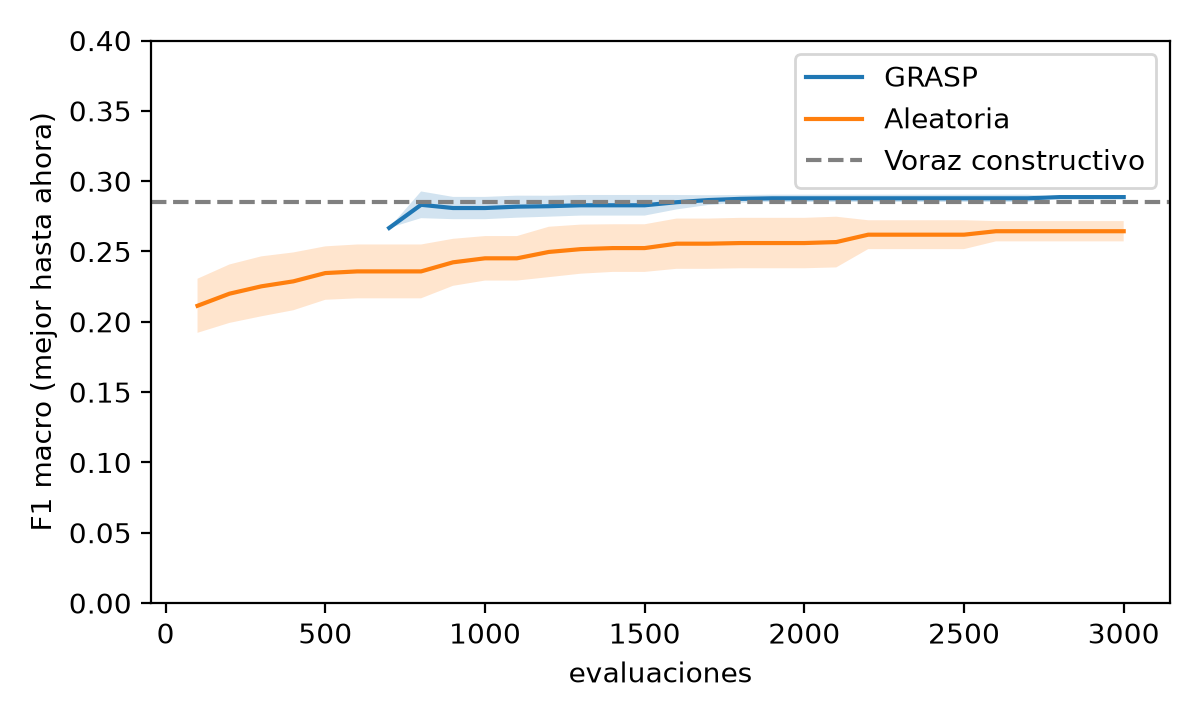
\includegraphics[width=\columnwidth]{convergencia.png}
		\caption{Mejor $\bar F_1$ acumulado frente a evaluaciones reales ($K=5$, $t_{\max}=80$\,ms; media $\pm$ desviaci\'on de 10 semillas).}
		\label{fig:conv}
	\end{figure}
	
	\subsection{Validaci\'on cruzada por organizaci\'on}
	En cada pliegue se optimiza con los otros cuatro y se eval\'ua en el reservado ($K=5$, $t_{\max}=80$\,ms, $\alpha=0{,}3$, 3.000 evaluaciones). La Tabla~\ref{tab:cv} resume los pliegues. Los valores var\'ian mucho entre pliegues: el techo de cada uno (todas las reglas sin enmascarar) va de 0,22 a 0,74. Las diferencias pareadas entre GRASP y el voraz son $-0{,}033$, $-0{,}159$, $+0{,}055$, $-0{,}044$ y $+0{,}138$ (media $-0{,}008$): no hay evidencia de que uno supere al otro. Entre GRASP y la aleatoria la media es $+0{,}032$ y gana en 3 de 5 pliegues. El voraz supera a la aleatoria en 4 de 5 (media $+0{,}040$).
	
	\begin{table}[t]
		\centering
		\caption{Validaci\'on cruzada (media $\pm$ desv. entre 5 pliegues)}
		\label{tab:cv}
		\footnotesize
		\begin{tabular}{lccc}
			\toprule
			M\'etodo & $\bar F_1$ & Precisi\'on & Cobertura \\
			\midrule
			Voraz constructivo & $0{,}311\pm0{,}137$ & 0,991 & 0,485 \\
			GRASP & $0{,}303\pm0{,}144$ & 0,954 & 0,312 \\
			Aleatoria & $0{,}271\pm0{,}109$ & 0,971 & 0,338 \\
			\bottomrule
		\end{tabular}
	\end{table}
	
	\subsection{Muestra manual sin referencia}
	De 36 fichas, 34 siguen la plantilla de AutoTrain y 2 son de formato libre. Se compar\'o cada valor extra\'ido con el texto de la ficha: las 36 son correctas. El intervalo de Wilson \cite{wilson} al 95\,\% es 90,4--100\,\%. En 4 fichas el extractor omiti\'o m\'etricas (RMSLE, varianza explicada, CodeBERT y columnas de otros conjuntos de datos). En total el extractor encuentra alguna m\'etrica en 1.725 de 2.057 fichas (84\,\%), 1.387 de ellas sin referencia, frente al 19,5\,\% de la cascada actual.
	
	\subsection{Aplicaci\'on a los modelos sin m\'etricas}
	Se aplicaron dos configuraciones a los 1.664 modelos sin valores num\'ericos en el \texttt{model-index} (126 sin README). La de GRASP ($K=6$, 80\,ms; $\bar F_1=0{,}340$, $P=0{,}995$ y cobertura 0,707 en la referencia) recupera m\'etricas en menos de 30 de ellos. Con todas las reglas en el orden fila, columna, l\'inea ($\bar F_1=0{,}384$, 170\,ms por ficha) se recuperan en 1.386 (83\,\%): 88\,\% de las fichas de clasificaci\'on de texto, 94\,\% de im\'agenes, 90\,\% de resumen, 95\,\% de clasificaci\'on de tokens y 91\,\% de traducci\'on; en generaci\'on de texto solo 9\,\%. Una inspecci\'on de 12 fichas al azar entre las 1.386 no mostr\'o valores ajenos a las m\'etricas del modelo.
	
	\section{An\'alisis y conclusiones}
	\textbf{Enmascaramiento.} En una versi\'on previa de 18 reglas, activarlas todas en el orden del cat\'alogo daba cobertura 0,374, frente a 0,801 con un orden adecuado (fila, columna, l\'inea); sin enmascarar tambi\'en 0,801. El orden de prioridad es entonces una decisi\'on real y no basta con activar todo.
	
	\textbf{M\'etodos.} Un voraz constructivo es una l\'inea base muy fuerte aqu\'i. GRASP lo iguala y, en la instancia peque\~na, alcanza el \'optimo exacto en todas las r\'eplicas. Su ventaja m\'as clara es con la restricci\'on de tiempo a 80\,ms, aunque de solo 0,004. Ambos superan a la b\'usqueda aleatoria en el conjunto completo. Fuera de muestra, la diferencia GRASP--voraz es ruido y GRASP tiene menor cobertura (0,312 frente a 0,485). Una posible explicaci\'on, no comprobada, es sobreajuste: el $F_1$ macro pesa por igual etiquetas con una o dos fichas, y una b\'usqueda m\'as intensa se ajusta a ese ruido.
	
	\textbf{Transferencia.} La configuraci\'on optimizada no se transfiere. Se ajust\'o sobre una referencia de similitud de oraciones y extracci\'on de caracter\'isticas, y con $K=6$ queda sin las reglas en l\'inea que usa el formato AutoTrain, que domina la poblaci\'on objetivo. Un l\'imite de $K$ pensado para el mantenimiento sacrifica as\'i casi toda la cobertura donde m\'as hace falta. La funci\'on objetivo debe incluir esa poblaci\'on, por ejemplo con los conjuntos validados de AutoTrain o con una ponderaci\'on por la distribuci\'on real de tareas.
	
	\textbf{Limitaciones.}
	(i)~La precisi\'on es una cota inferior, porque el cuerpo puede traer m\'etricas correctas ausentes del \texttt{model-index}.
	(ii)~En las fichas AutoTrain \texttt{model-index} y cuerpo reportan mediciones distintas (por ejemplo, ROUGE-2 de 12,47 frente a 10,90), lo que debilita la independencia de la referencia.
	(iii)~Una sola organizaci\'on aporta 236 de las 390 fichas y cerca del 75\,\% de las m\'etricas de referencia de la partici\'on de entrenamiento usada en el ajuste.
	(iv)~Los pliegues son muy desiguales y varias etiquetas tienen una sola ficha.
	(v)~Los hiperpar\'ametros se ajustaron en una partici\'on distinta de la validaci\'on cruzada, con posible fuga leve; el efecto es peque\~no porque $\alpha$ no es sensible.
	(vi)~Los tiempos dependen de la implementaci\'on y la m\'aquina.
	(vii)~La muestra manual es casi toda AutoTrain y no estima la precisi\'on en formato libre.
	
	\textbf{Trabajo siguiente.} La Entrega 4 incorpora un algoritmo gen\'etico y una prueba estad\'istica pareada sobre m\'as instancias, un cat\'alogo mayor que ampl\'ie el techo de 0,383, una ponderaci\'on por ficha para reducir el peso de las organizaciones dominantes y de las etiquetas diminutas, y una funci\'on objetivo que incluya los modelos AutoTrain.
	
	\begin{thebibliography}{1}
		\bibitem{mitchell} M. Mitchell \emph{et al.}, ``Model cards for model reporting,'' in \emph{Proc. Conf. Fairness, Accountability, and Transparency (FAT*)}, Atlanta, GA, USA, 2019, pp. 220--229.
		\bibitem{feo} T. A. Feo and M. G. C. Resende, ``Greedy randomized adaptive search procedures,'' \emph{J. Global Optim.}, vol. 6, no. 2, pp. 109--133, 1995.
		\bibitem{wilson} E. B. Wilson, ``Probable inference, the law of succession, and statistical inference,'' \emph{J. Amer. Statist. Assoc.}, vol. 22, no. 158, pp. 209--212, 1927.
	\end{thebibliography}
	
\end{document}